\section{Structural Cases and Refinement Diagnostics}
\label{sec:scoped-sufficiency}

\subsection{Two comb components}
Let $C_a$ be a full binary comb with $a$ leaves; $C_1$ is a leaf.
For $F=(C_a,C_b)$ with $a\ge b\ge1$, the height is $m=a$ and
$N=2a+2b-2$. Depth coloring $C_a$ gives $(1,2,\ldots,2)$.
Designate its root color by $c_0$.

If $b=1$, give the other leaf color $c_0$, obtaining all loads two,
including $a=b=1$. If $b\ge2$ and $a\ge2b-2$, the average lower bound
is three. In $C_b$, color its two terminal sibling leaves $c_0$ and
give each of the other $2b-3$ vertices a distinct color. The inequality
$2b-3\le a-1$ provides enough remaining colors. Only incomparable
siblings share a color in $C_b$, and all combined loads are at most
three. Finally, if $a<2b-2$, then $3<N/a<4$; depth coloring both
components with the same palette gives capacity at most four.
Each construction attains $\lceil N/a\rceil$ in one pass. Since
$\lceil N/a\rceil\le B_{\rm joint}\le U^*$, these constructions certify
optimality for two comb components.

\subsection{A strict gap at arbitrarily growing height}
\label{sec:wrapper-strictness}
For a two-component full binary forest $F=(A,B)$, let
$W(F)=((A,B),L)$: introduce a new parent $r$ above $A,B$ and a new
outside leaf $z$. If $F$ has $N$ records, $n$ leaves, and height $m$,
then $W(F)$ has $N+2$ records, $n+1$ leaves, and height $m+1$.

\begin{proposition}[Wrapper invariance]
\label{prop:supp-wrapper-invariance}
With the palette fixed to each forest's height,
\begin{align}
 U^*(W(F),m+1)&=U^*(F,m),\label{eq:supp-wrapper-optimum}\\
 B(W(F))&=B(F),\label{eq:supp-wrapper-average}\\
 B_{\rm hier}(W(F))&=B_{\rm hier}(F),
 \label{eq:supp-wrapper-individual}\\
 B_{\rm joint}(W(F))&=B_{\rm joint}(F).
 \label{eq:supp-wrapper-joint}
\end{align}
\end{proposition}

\begin{proof}
A full binary component of height $m$ has at least $2m-1$ vertices;
the other component is nonempty. Thus $N\ge2m$ and $U^*\ge B\ge2$.
Extend an optimal coloring of $F$ by assigning $r,z$ one new color of
load two. Conversely, $r$ conflicts with every old vertex, so any
$(m+1)$-coloring of $W(F)$ restricts to an $m$-coloring of $F$.
This proves~\eqref{eq:supp-wrapper-optimum}.

The descendants of $r$ are the old global context. Every old context
retains its records and available colors because its depth and the
total palette both increase by one. The new leaf's context is empty.
The only new average is $\lceil(N+2)/(m+1)\rceil\le B(F)$, since
$N\le mB(F)$ and $2\le B(F)$. This proves~\eqref{eq:supp-wrapper-average}.

It remains to check the new global anchored paths. For $(z)$, the
individual and joint capacities both equal $n+1$, giving the candidate
$\lceil(N+1-n)/m\rceil\le\lceil N/m\rceil$. For $(r)$, both capacities
are two, giving $\lceil N/m\rceil$.

Every longer path is $(r,P)$, with $P$ an old global path of length
$1\le k<m$. Write $S(P)$ for its old sum of individual capacities.
The outside leaf increases each old anchor's individual capacity by
one, and $r$ has capacity two. Its new test is therefore
\begin{equation}
 \left\lceil\frac{N-S(P)-k}{m-k}\right\rceil
 \le \left\lceil\frac{N-S(P)}{m-k}\right\rceil.
 \label{eq:supp-wrapper-individual-test}
\end{equation}
For the joint test, $r$ and $z$ contribute two records; all old side
forests retain their available suffix palettes. The new joint
capacity is exactly $2+J(P)$, so its ratio equals the old ratio
$\lceil(N-J(P))/(m-k)\rceil$. Paths reaching the last depth have
zero denominator and contribute no test, as established above.
All old tests remain through the descendant context of $r$ and the
unchanged old contexts. These cases exhaust the new tests, proving
the two remaining equalities.
\end{proof}

To obtain a strict family, let $L$ be a leaf, $C=(L,(L,L))$,
$P=((L,L),(L,L))$, and $F_0=(C,(L,(C,P)))$. Then
$N_0=20$, $n_0=11$, and $m_0=5$. Anchor the root of the second
component and its nonleaf child. Their joint capacity is
$2+\beta_2(C)+\beta_1(L)=2+4+1=7$, giving the bound
$\lceil(20-7)/3\rceil=5$. A proper preorder coloring on colors
$1,\ldots,5$ is
\begin{equation}
 \begin{aligned}
 \varphi_0=(\, &3,5,4,5,5,\;3,4,5,1,2,\\
              &4,2,2,4,2,1,1,2,1,1\,).
 \end{aligned}
 \label{eq:supp-wrapper-seed-coloring}
\end{equation}
Its loads are $(5,5,2,4,4)$, proving $U^*=5$.

For completeness, $B_{\rm hier}=4$ can be checked without an exact
solver. Index the virtual root by zero and real vertices in preorder
by $1,\ldots,20$. For each nonempty context, take the minimum slack
at capacity four over its average test and all individual-anchor tests:
\begin{equation}
 \begin{split}
 \sigma_x=\min\Bigl\{4q_x-N_x,\qquad\qquad\qquad\quad\\
 \min_{P:\,1\le|P|<q_x}
 \Bigl[\sum_{v\in P}a_{x,v}+4(q_x-|P|)-N_x\Bigr]\Bigr\}.
 \end{split}
 \label{eq:supp-seed-slack}
\end{equation}
The nonempty contexts, grouped only to fit the column, give
\begin{equation}
 \begin{array}{c|rrrrr}
 x&0&1&3&6&8\\ \hline
 \sigma_x&0&9&8&0&0\\[2pt]
 x&9&11&14&15&18\\ \hline
 \sigma_x&2&2&1&2&2
 \end{array}.
 \label{eq:supp-seed-slack-values}
\end{equation}
All tests are satisfied at four and the global average equals four.
Hence $B=B_{\rm hier}=4<B_{\rm joint}=U^*=5$.

Iterating the wrapper yields, for every $t\ge0$,
\begin{align}
 F_t&=W^t(F_0),\\
 (N_t,n_t,m_t)&=(20+2t,11+t,5+t),\label{eq:supp-wrapper-family}\\
 B(F_t)&=B_{\rm hier}(F_t)=4,\\
 B_{\rm joint}(F_t)&=U^*(F_t,m_t)=5.
 \label{eq:supp-wrapper-family-gap}
\end{align}
Assign one new color of load two per wrapper to construct the witness
in linear time. Padding each skeleton leaf's binary path with zeros
embeds the forest in a common-height SMT. For fixed physical height
$h$, this requires $5+t\le h$; the infinite family allows $h$ to grow.

\subsection{Finite checks of the structural statements}
The complete profile census contains 1323 unordered, unlabeled full
binary skeletons with 2--14 leaves and 2115 with 15--16 leaves, all
with root-excluded height $m\le6$. Their two root-child trees are the
record forest. Exact optima were computed from the context bound
upward, independently of the joint bound. All 3438 have
$B_{\rm joint}=U^*$; the joint term closes 13 gaps left by
$B_{\rm hier}$, with 12 two-anchor and one three-anchor witnesses.
The 13 exact layouts pass all 168 occupied-target SMT checks.
The $O(Nm)$ evaluator reproduces all 3438 frozen bound values.

Independent checks validate 210 comb pairs with $1\le b\le a\le20$
and 4410 SMT proofs. Six fixed wrapper counts
$t\in\{0,1,2,5,10,25\}$ give 109 further proofs, including mutation
rejection and equality of the reconstructed support forest with the
abstract shape. The comb and wrapper statements follow from their
constructions; the census does not establish general joint sufficiency.

\subsection{Exact moves on a bounded selected palette}
\label{sec:construction-neighborhood}
The refinement study starts from the original AB with a 20-scan budget.
A pair control optimizes unions of two-color Kempe components by
subset-sum. The three-color variant recolors the induced forest on
three selected classes; the four-color stage follows if needed.
Unselected vertices retain their colors.

For a selected palette $K$, link each selected vertex to its closest
selected ancestor. This compression preserves the induced ancestor
relation, even when the projected forest has more roots or children.
Let $\mathcal P_K(T_v)$ contain all feasible load vectors indexed by
$K$ for the projected rooted subtree $T_v$. The exact recurrence is
\begin{equation}
 \mathcal P_K(T_v)=
 \bigcup_{c\in K}
 \left\{\mathbf e_c+\sum_{w}p_w:
 p_w\in\mathcal P_{K\setminus\{c\}}(T_w)\right\},
 \label{eq:supp-selected-palette-dp}
\end{equation}
with omitted coordinates extended by zero. Empty forests have the
zero vector; a nonempty tree has no profile on an empty palette.
A root consumes one color unavailable to its descendants. Conversely,
child witnesses using the remaining palette combine independently.
Induction therefore enumerates precisely all profiles, and summing
root profiles handles the forest. Retaining predecessor choices
recovers a witness. Outside vertices use colors outside $K$, so the
move preserves cross-boundary properness.

Kempe exchanges are established coloring operations~\cite{kempeequivalence}.
The ancestor graph is $(m-1)$-degenerate: a deepest remaining vertex
has only its remaining ancestors as neighbors. Proposition~2.4 of
that reference implies Kempe connectivity of its proper $m$-colorings.
The connecting paths need not preserve capacity. Similarly, minimizing
each child profile separately is insufficient: two seven-node perfect
components each have locally best profile $(1,3,3)$, whose best merge
has capacity six, while profiles $(1,2,4)$ permit loads $(5,4,5)$.
These facts explain why the study retains complete small profile sets.

The prototype is limited to $N\le30$, $m\le6$, 100 moves per stage,
20000 profiles per merge, and 10000 cached rooted subproblems; none
of these limits was reached in the reported cohorts. Independent
checks compare 44 complete profile sets with labeled brute force and
validate 3542 projections. Four methods verify 198628 SMT proofs
across the two cohorts. The method is a bounded structural diagnostic,
and its exact move computation is not a scalable optimizer claim.

% Generated from frozen structural results. Requires booktabs and graphicx.
\begin{table*}[t]
\centering\small
\caption{Exact structural gaps. Each cell is base / holdout; cohorts contain 1323 / 2115 shapes. $\Delta=U-\mathrm{OPT}$ is an integer record count and $r=\Delta/\mathrm{OPT}$. Every shape has equal weight.}
\label{tab:structural-exact-gaps}
\begin{tabular}{lrrrr}
\toprule
Method & OPT hits & Mean $\Delta$ & Max $\Delta$ & Max $r$ (\%)\\
\midrule
First-fit & 96 / 20 & 2.054 / 3.022 & 6 / 8 & 100.0 / 140.0\\
AB & 1123 / 1780 & 0.151 / 0.158 & 1 / 1 & 25.0 / 20.0\\
AB + pair & 1125 / 1796 & 0.150 / 0.151 & 1 / 1 & 25.0 / 20.0\\
AB + 3 & 1314 / 2073 & 0.007 / 0.020 & 1 / 1 & 25.0 / 20.0\\
AB + 3$\to$4 & 1321 / 2112 & 0.002 / 0.001 & 1 / 1 & 25.0 / 20.0\\
Exact OPT & 1323 / 2115 & 0.000 / 0.000 & 0 / 0 & 0.0 / 0.0\\
\bottomrule\end{tabular}\end{table*}
First-fit uses the smallest available ancestor color and is depth coloring on these skeletons. Both cohorts use the same algorithms and independently checked canonical skeletons and record-parent forests. These results measure structural optimality gaps; they are not PIR timings.
The final five failures are S0606, S0710, H1199, H1265, and H1285. Each has $U-\mathrm{OPT}=1$; their exact relative gaps are $1/4$, $1/4$, $1/5$, $1/5$, and $1/6$, respectively. This finite observation does not imply a constant additive approximation guarantee.
\begin{figure*}[t]\centering
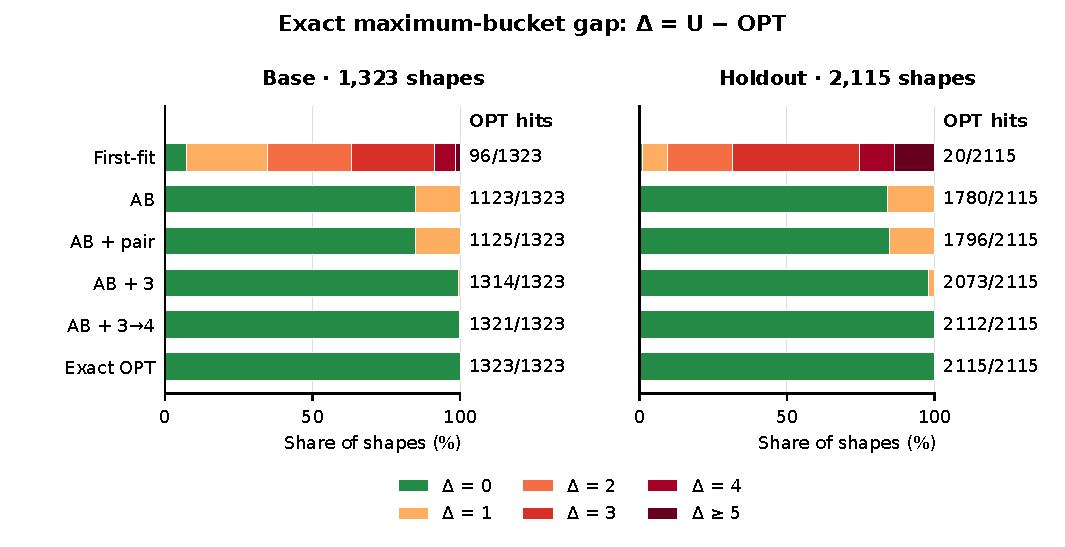
\includegraphics[width=\textwidth]{figures/absolute_gap_distribution_compact.pdf}
\caption{Exact integer gap distribution on the two frozen censuses; gaps of five or more are grouped. Green denotes an attained optimum; labels give exact hit counts. The final five positive gaps are all one record, but the worst relative gaps remain 25\% and 20\%. These are structural counts, not PIR costs or deployment success rates.}
\label{fig:structural-gap-distribution}\end{figure*}


\subsection{The five residual states}
\label{sec:plateau-diagnostic}
All five failures have $N=mL$, where $L=U^*$, and descending loads
$(L+1,L,\ldots,L,L-1)$. A strictly smaller sorted integer vector with
the same sum must be $(L,\ldots,L)$. Indeed, reducing the first entry
forces every entry to be at most $L$; keeping that entry and first
reducing a later one leaves too little total mass. Thus a direct
improvement must include both the overfull and underfull color.

Across these states there are 27 four-color palettes containing both
colors. Fix all outside colors. Every selected forest has $4L$ records.
For each palette, a stored anchored path of length $k<4$ has
$J(P)=kL-1$, evaluated with four available colors. Its capacity test
would require
\begin{equation}
 4L\le J(P)+(4-k)L=4L-1,
 \label{eq:supp-plateau-obstruction}
\end{equation}
which is impossible. Using the projection's smaller height in place
of its four allowed colors would not justify this conclusion.
A move on fewer colors could be extended to a four-color palette;
hence no move on at most four colors reaches the optimum directly.
Every optimal recoloring changes the membership of at least five
classes, counting both source and destination labels.

For each of the five states, a valid four-color move preserving the
sorted loads is followed by a strict four-color move attaining all
loads $L$. The minimum number of at-most-four-color moves is therefore
exactly two for these states. Independent verification checks the
27 inequalities and 222 SMT proofs across initial, neutral, and final
layouts. This targeted diagnosis explains the frozen failures; it
does not alter the reported cohort success rates or establish a
general convergence theorem.
